
%(BEGIN_QUESTION)
% Copyright 2010, Tony R. Kuphaldt, released under the Creative Commons Attribution License (v 1.0)
% This means you may do almost anything with this work of mine, so long as you give me proper credit

Describe one practical improvement a technician could impart to this poor wiring installation.  Be as specific as you can in your answer, highlighting areas in the photograph if necessary:

$$\includegraphics[width=15.5cm]{i04549x01.eps}$$

Try to not laugh too hard -- someone actually got paid to build this!

\underbar{file i04549}
%(END_QUESTION)





%(BEGIN_ANSWER)

Any of the following are acceptable answers:

\begin{itemize}
\item{} Better separation of power and signal conductors
\item{} Use wire duct or tie-downs to marshal wiring neater (avoiding crossover)
\item{} No more than one compression terminal per lug on side-mounted switch (use terminal block to double up connections)
\item{} Discard wire nuts in favor of connections at terminal block
\item{} Shorten wires (or stuff excess in conduit) to avoid cluttering loops of wire
\end{itemize}

%(END_ANSWER)





%(BEGIN_NOTES)


%INDEX% Good practices, wiring: example of bad wiring

%(END_NOTES)

